%!TEX root=../sig-alternate-sample.tex

\section{Experiments}
\subsection{Data Preprocessing}
Different data source supply data with different dimensions. So, we must normalize the data to make them comparable. 
Given a line $S = [(d_1, v_1), \cdots, (d_n, v_n)]$, we can normalize its value using the Min-Max scaling method:
\begin{equation}
	Norm(S) = [(d_1, \frac{v_1 - v_min}{v_max - v_min}), \cdots, (d_n, \frac{v_n - v_min}{v_max - v_min})]
\end{equation}

Normalization is recommended so that the distance between two lines is invariant to value scaling and shifting. In the next part, we will refer the $S$ as $Norm(S)$. 

We have prepared two categories of dataset: economic indicators and the electricity consumption. The first dataset is crawled from the website of National Bureau of Statistics of China. It consists of various of economic indicators monthly in consumer price, industry, fixed assets investment and domestic trading etc, that lasts about recent fifteen years. The second dataset is about the electricity consumption of each day in the east China, which includes Anhui, Fujian, Shanghai, Jiangsu, Zhejiang. In order to ensure the comparability, we sum the daily record of electricity consumption into one new record representing the electricity consumption of the corresponding month. 

We implemented the proposed similarity method as described in the previous sections and presented the experimental results. Our experiments were taken on a MAC OS X at 2.7 GHz with 8GB RAM.

\subsection{Similarity}
Firstly, we will compare the top 10 indicators that mostly close to the electricity consumption. Table~\ref{tab:topindi} shows the top-ten indicators in Anhui Provinces. We could use the Jaccard similarity to evaluate how the results of different methods are relevant. Given set A and B, 
\begin{equation}
	Jaccard(A, B) = \frac{\texttt{|A intersect B|}}{\texttt{|A union B|}}
\end{equation} 
where the $|A|$ notates the count of element in set $A$. Obviously, the value would increase if there are more elements overlapping in these two sets. We could use the DTW method as baseline to evaluate the Jaccard similarity between the results of these methods in different provinces. From the figure~\ref{fig:Jaccard}, we can see that in the top ten indicators, the jaccard similarity of DTW and other methods lie from 0.25 to 0.43, espically the Zhejiang Province, of which results are higher than other provinces. The fact that we can get same indicators in the top ten indicators gives a strong support to the viewpoint that these indicators have a relationship with the electricity consumption.

\begin{figure}
	\centering
	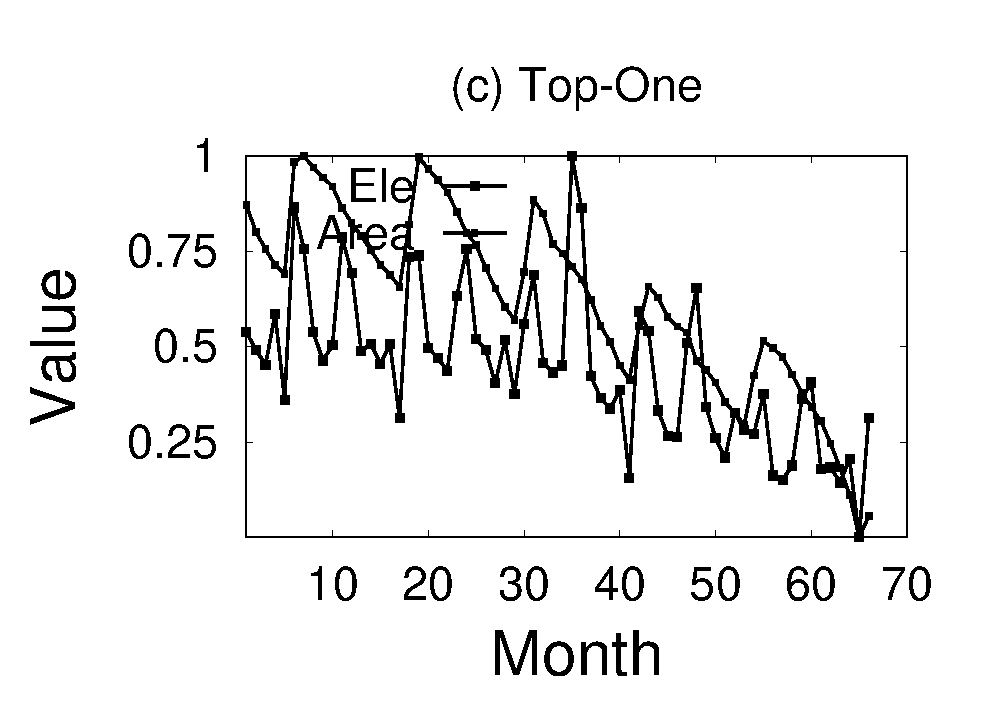
\includegraphics[height=2in, width=1.9in]{area-ele}
	\caption{AreaSim Top One}
	\label{fig:AreaSim}
\end{figure}

\begin{figure}
	\centering
	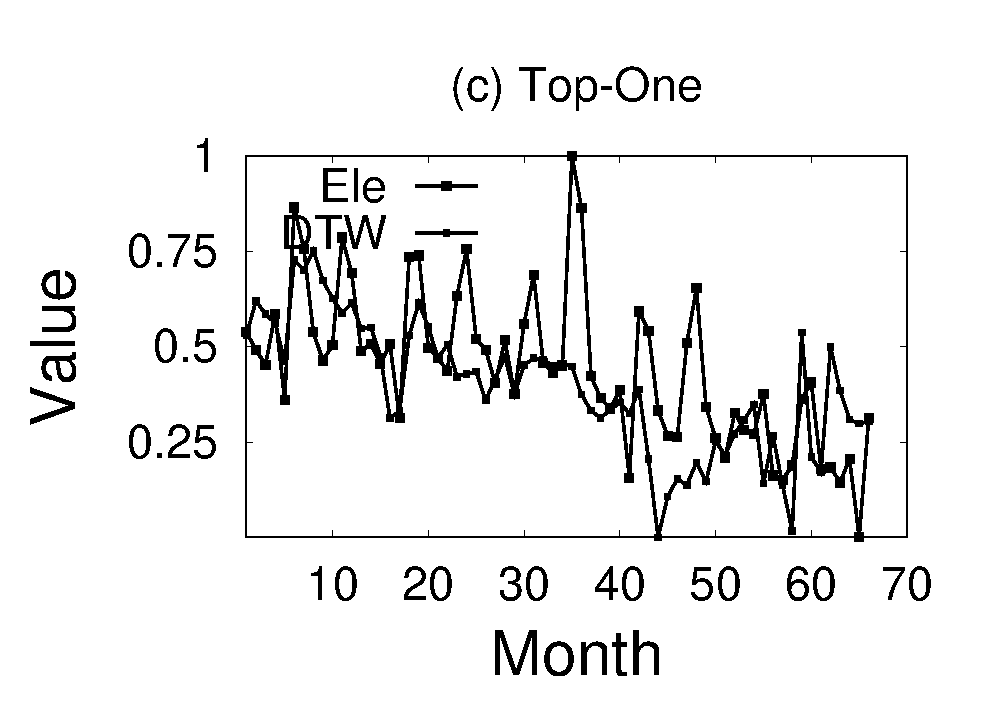
\includegraphics[height=2in, width=1.9in]{dtw_ele}
	\caption{DTW Top One}
	\label{fig:DTW}	
\end{figure}

\begin{figure}
	\centering
	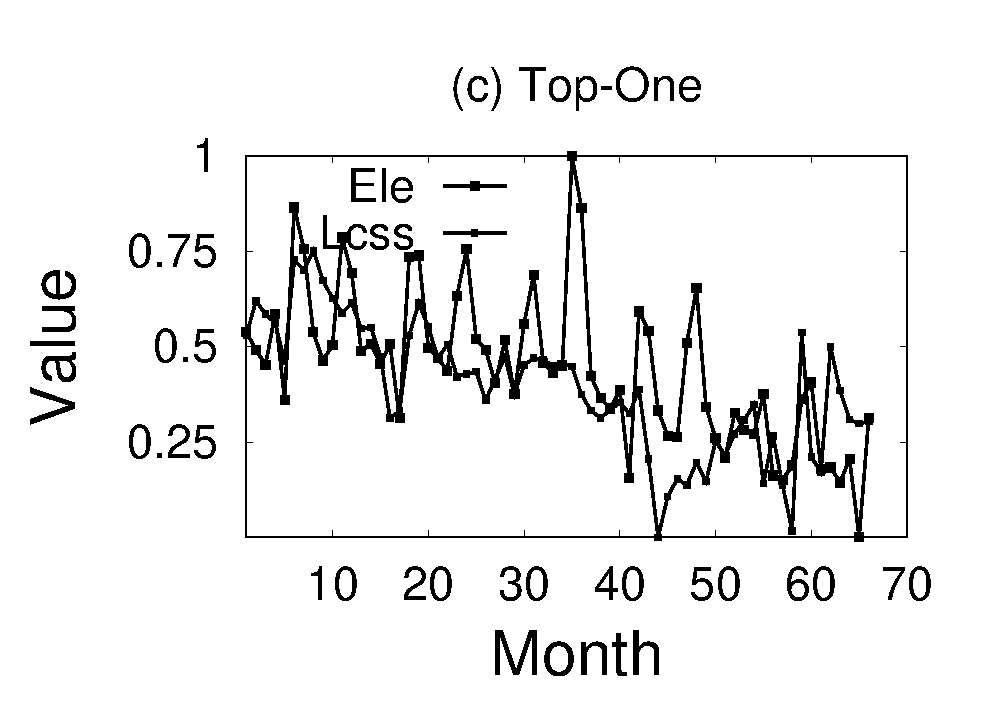
\includegraphics[height=2in, width=1.9in]{lcss-ele}
	\caption{LCSS Top One}
	\label{fig:LCSS}
\end{figure}

\begin{figure}
	\centering
	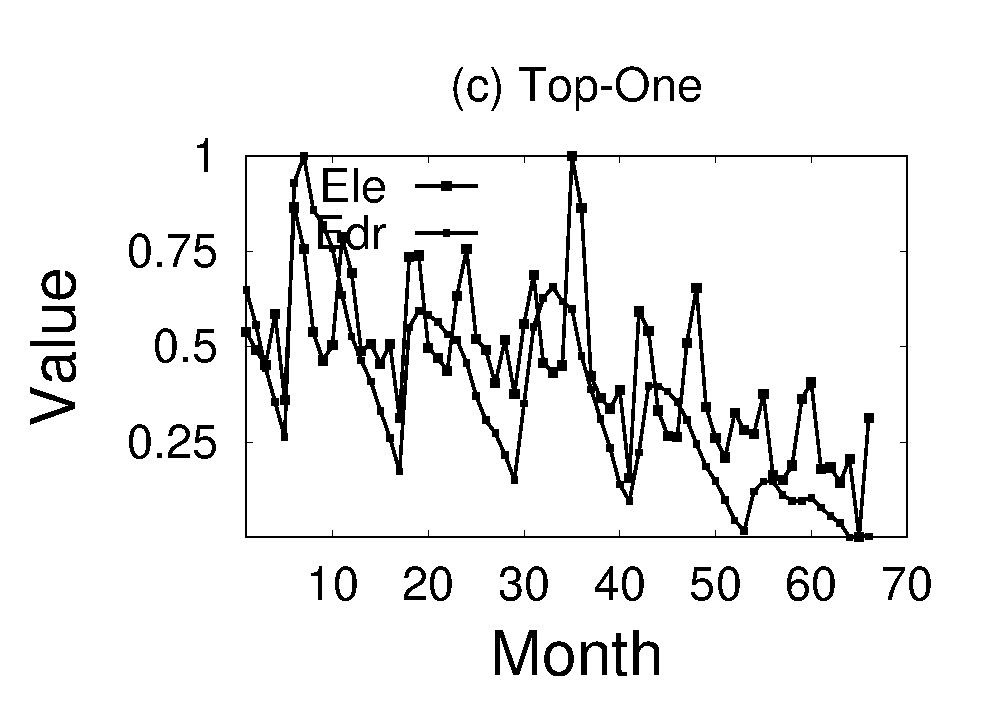
\includegraphics[height=2in, width=1.9in]{edr-ele}
	\caption{EDR Top One}
	\label{fig:EDR}
\end{figure}

\begin{figure}
	\centering
	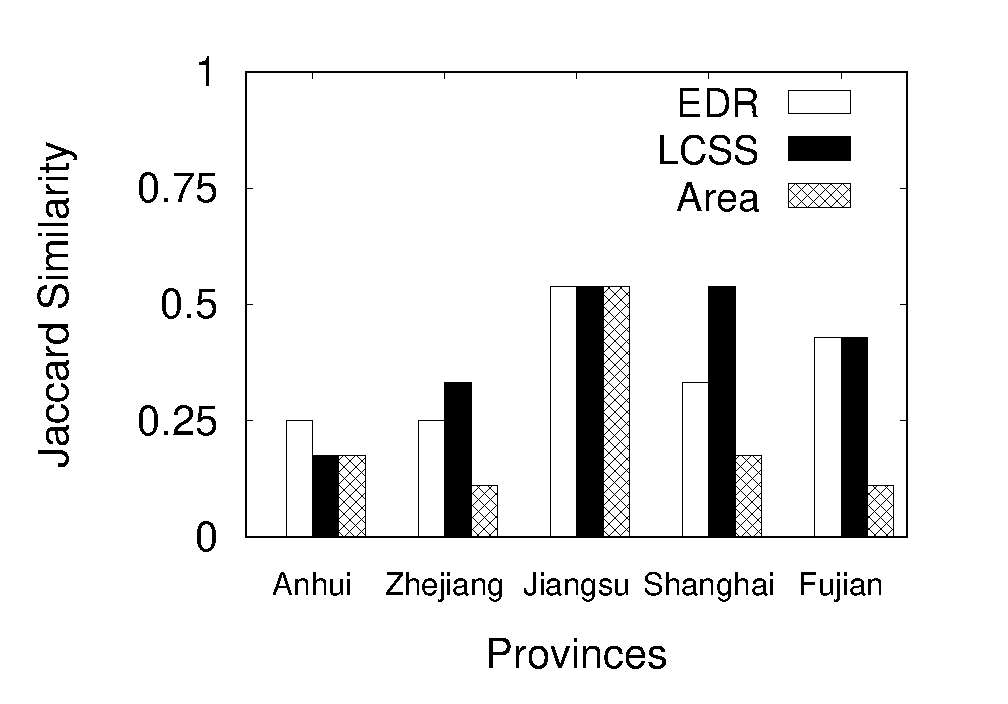
\includegraphics[height=2in, width=1.9in]{dtw_jaccard_similarity}
	\caption{Jaccard Similarity Based on DTW}
	\label{fig:Jaccard}
\end{figure}

\begin{table*}
\centering
\caption{Top 10 Relevant Indicators}
\label{tab:topindi}

\begin{tabular}{|p{3cm}|c|p{3cm}|c|p{3cm}|c|p{3cm}|c|} \hline
	\multicolumn{2}{|c|}{DTWSIM} & \multicolumn{2}{|c|}{LCSSSIM} &\multicolumn{2}{|c|}{EDRSIM} & \multicolumn{2}{|c|}{AreaSIM}\\ \hline
	Construction area of commercial premises\_Cumulative growth(\%) & 0.8944 & The purchase of equipment and instruments in fixed assets investment\_cumulative growth(\%) & 0.9104 & The purchase of equipment and instruments in fixed assets investment\_cumulative growth(\%)& 0.9516 & Residential construction area\_cumulative growth(\%)& 0.8822\\ \hline
	Stock\_cumulative growth(\%) & 0.8930 & Commercial housing construction are\_cumulative growth(\%) & 0.8529 & Commercial housing construction are\_cumulative growth(\%) & 0.9104 & Commercial housing construction are\_cumulative growth(\%) & 0.8817\\ \hline
	Residential construction area\_cumulative growth(\%) & 0.8908 & The amount of investment in fixed assets\_cumulative growth(\%)& 0.8507 & The amount of investment in fixed assets\_cumulative growth(\%) & 0.9032
 & Value added tax payable\_cumulative growth(\%) & 0.8804\\ \hline
	Real estate construction area\_cumulative growth(\%) & 0.8890 &Total current assets\_cumulative growth(\%) & 0.8382 & Total current assets\_cumulative growth(\%) & 0.8955 & The finished product\_cumulative growth(\%) & 0.8787\\ \hline
	Construction area of commercial housing\_Cumulative growth(\%) & 0.8884 & Management Expenses\_Cumulative growth(\%) & 0.8382
& The finished product\_Cumulative Growth(\%) & 0.8955 & Residential construction area\_Cumulative growth(\%) & 0.8749\\ \hline
	Taxes and surcharges of principal operations\_Cumulative growth(\%) & 0.8884 & Accounts Receivable \_ Cumulative Growth (\%) &0.8235 & Accounts Receivable \_ Cumulative Growth (\%) & 0.8805 & Investment in fixed assets completed \_ cumulative growth (\%) & 0.8676
\\ \hline
	Total Assets \_ Cumulative Growth (\%) & 0.8854 & Finished products\_Cumulative growth& 0.8235& Management Expenses\_Cumulative growth&0.8805 & Construction area of office buildings\_Growth(\%) &0.8623\\ \hline
	The purchase of equipment and instruments in fixed assets investment\_cumulative growth(\%) & 0.8841 &Total losses of loss-making enterprises\_Cumulative growth(\%) & 0.8235 &Total losses of loss-making enterprises\_Cumulative growth(\%)&0.8805 &Total losses of loss-making enterprises\_Cumulative growth(\%) &0.8618\\ \hline
	Accounts Receivable \_ Cumulative Growth (\%)& 0.8836& Completed area of commercial premises \_ Cumulative growth (\%) & 0.8235&Residential construction area\_cumulative growth(\%) & 0.8805 &Accounts Receivable \_ Cumulative Growth (\%)& 0.8559\\ \hline
	Total Liabilities \_ Cumulative Growth (\%)& 0.8830 & Residential construction area\_cumulative growth(\%)&0.8088 & Interest Expenditure \_ Cumulative Growth (\%)&0.8805 & The purchase of equipment and instruments in fixed assets investment\_cumulative growth(\%) & 0.8521\\ \hline
\end{tabular}
\end{table*}

\subsection{Lagging}
We have the dataset of electricity consumption and economic indicators lasting for sixty seven months. As is known, economic activities has 
periodicity, which is usually less than one year. Meanwhile, most of our economic indicators are evaluated monthly, so we should view one month as time unit. Taking our data as time series, We extract the middle part of our data intercepting the first last twelve month. And then, keeping the length of electricity consumption data, we move the economic indicator data forward and backward, getting different similarity, from which we could get the largest similarity. The moving month responding to the largest similarity is the lagging time offset we are seeking for. From the fig~\ref{fig:lagdis}, we can see that, different provinces has different lagging distribution.
 
Different lagging time offsets has different instructions for prediction of economic tendency and electricity consumption. The negative lagging time-offset value means that the current electricity consumption has a closer relationship with the economic indicators if we chose the later economic indicators. Therefore, we can predict the later economic indicators using current electricity consumption. Otherwise, if the lagging time-offset value is positive, we can predict the electricity consumption using current economic indicators.   
\begin{figure}
	\centering
	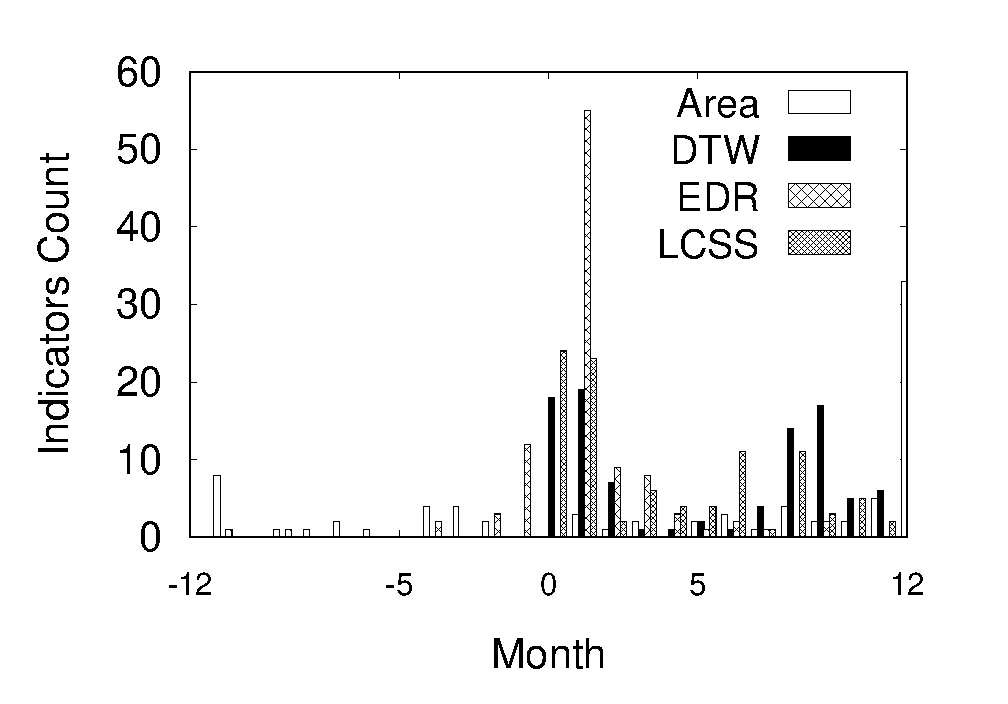
\includegraphics[height=1in, width=2in]{anhui_lag_dis}
	\caption{Anhui Lagging Time Distribution}
	\label{fig:anhui_lag}
\end{figure}

\begin{figure}
	\centering
	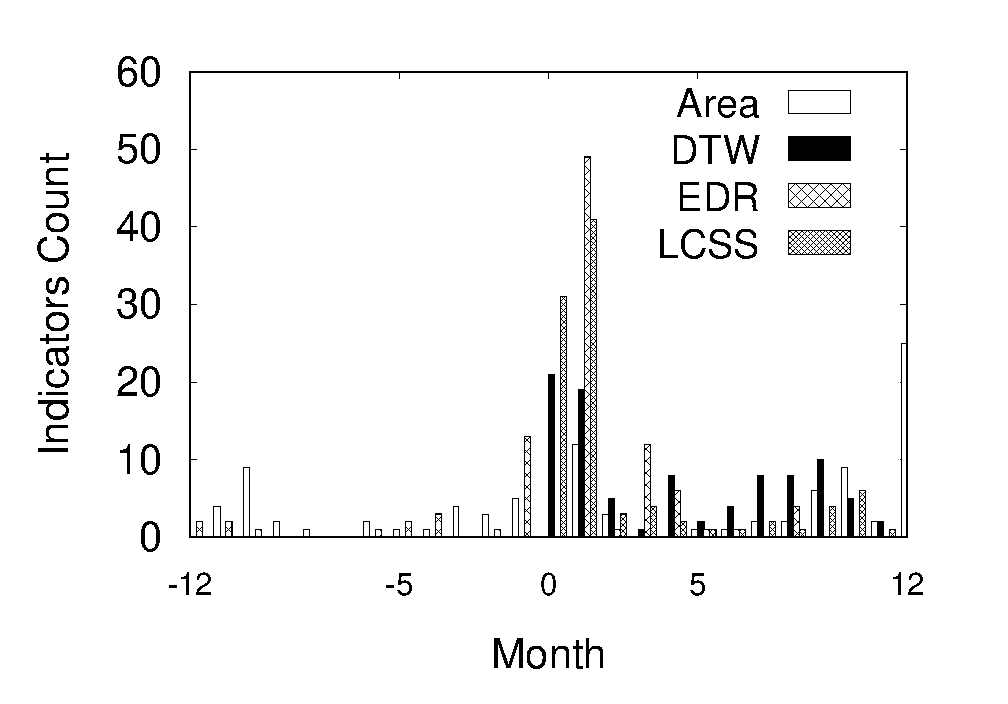
\includegraphics[height=1in, width=2in]{fujian_lag_dis}
	\caption{Fujian Lagging Time Distribution}
	\label{fig:fujian_lag}
\end{figure}

\begin{figure}
	\centering
	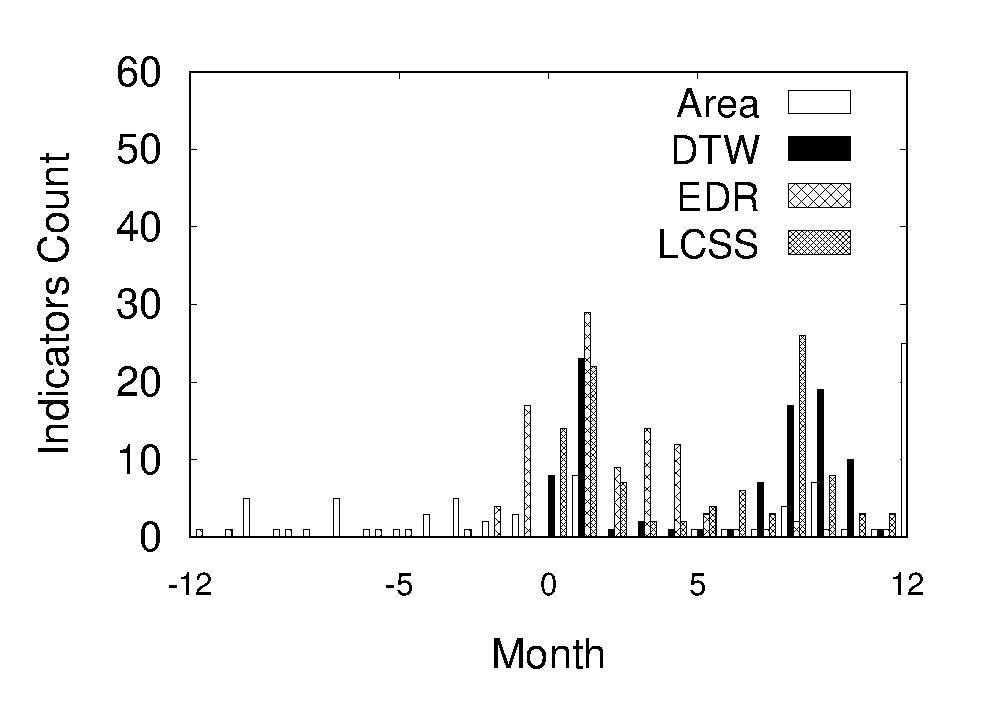
\includegraphics[height=1in, width=2in]{jiangsu_lag_dis}
	\caption{Jiangsu Lagging Time Distribution}
	\label{fig:jiangsu_lag}
\end{figure}

\begin{figure}
	\centering
	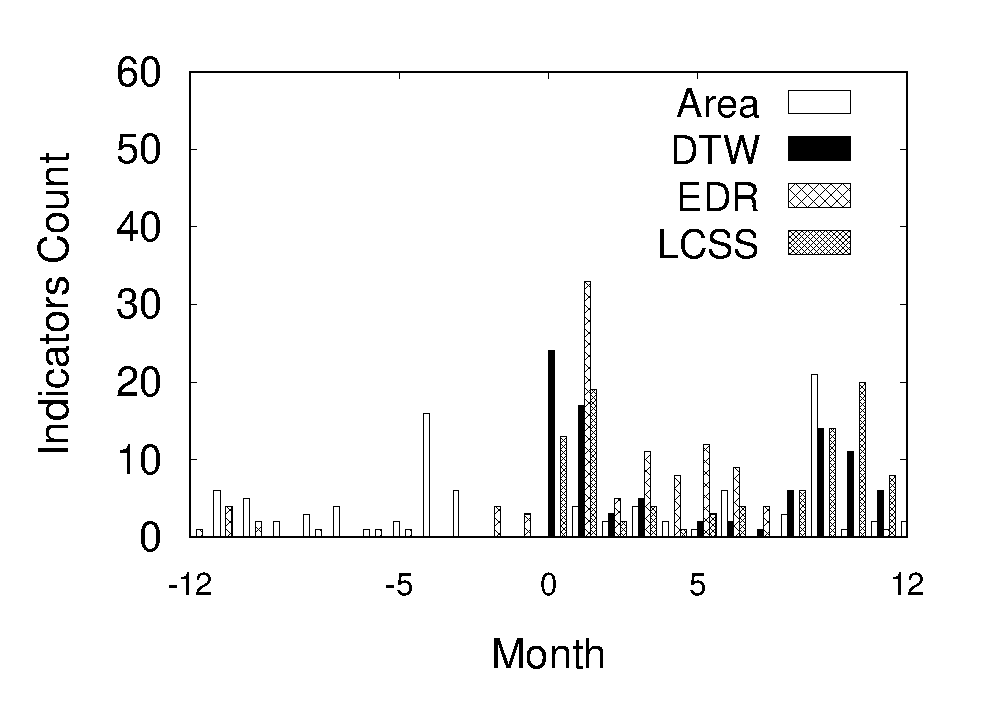
\includegraphics[height=1in, width=2in]{shanghai_lag_dis}
	\caption{Shanghai Lagging Time Distribution}
	\label{fig:shanghai_lag}
\end{figure}

\begin{figure}
	\centering
	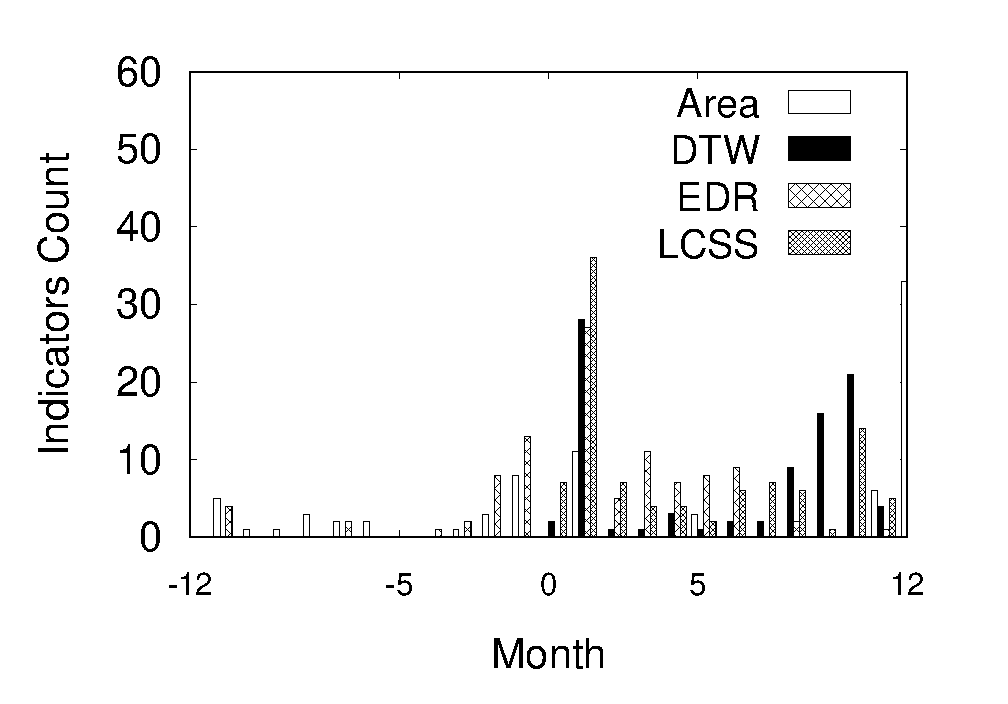
\includegraphics[height=1in, width=2in]{zhejiang_lag_dis}
	\caption{Zhejiang Lagging Time Distribution}
	\label{fig:zhejiang_lag}
\end{figure}